\documentclass[a4]{article}
\usepackage{gnuplottex}
\usepackage{csvsimple}
\usepackage{subcaption}
\usepackage{amsmath}
\usepackage{graphicx}
\usepackage{epstopdf}
\usepackage{float}

\graphicspath{ {./test_data/} }

\title{COMP26120 Lab 5 Report}
\author{Ziyi Li}

\begin{document}
\maketitle
Written with assistance from chatGPT

\section{What makes a problem hard for Dynamic Programming?}

\subsection{Hypothesis}

When using a dynamic programming algorithm to solve the knapsack problem, there should be a positive relation between the backpack's size and the program's runtime, when the input data size is fixed. This means that the program takes more time to process when the knapsack size increases.

\subsection{Design}

In order to prove the hypothesis, when designing the experiment, I set the number of items to be the same. I set up a total of two sets of experiments, 10,000 items and 5,000 items. \\

\noindent All input data are generated by script provided (kp\_generate.py). For each value of knapsack capacity, two sets of item data were generated to reduce errors in the experimental results. The ranges of size are between 500 to 15000 when items size is 10000 and 500 to 5000 when items size is 5000, both with spacing 500. The program used here is dp\_kp.py. In order to ensure that the output does not affect the running time of the program, all outputs are turned off. Python Jupyter Notebook is used here to run test and collect data.

\subsection{Results}
\begin{figure}[H]
    \begin{minipage}{0.48\textwidth}
    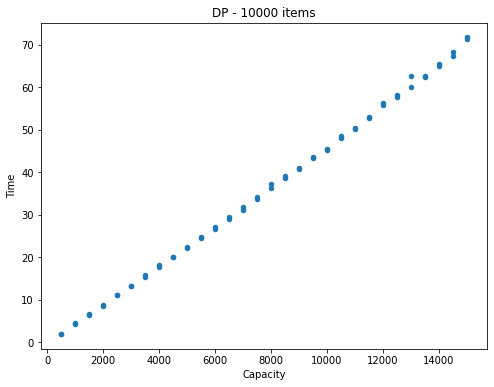
\includegraphics[width=0.95\textwidth]{dp-10000.png}
    \caption{10000 Items}
    \end{minipage}
    \begin{minipage}{0.48\textwidth}
        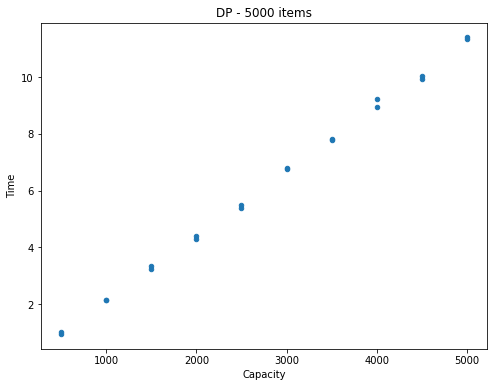
\includegraphics[width=0.95\textwidth]{dp-5000.png}
        \caption{5000 Items}
        \end{minipage}
\end{figure}


\subsection{Discussion}

According to the experimental results, we can observe a direct proportionality between the knapsack capacity and the runtime of the program. This means that as the knapsack capacity increases, the program's running time also increases proportionally. This is due to the amount of data that the program needs to process also increasing, so more time is required to calculate the solution.\\

\noindent This shows that the hypothesis holds. Therefore we can conclude that the larger knapsack size makes the knapsack problem more difficult to solve.\\

\noindent However in the situation when the capacity of the knapsack is greater than the number of items, all items can be packed into the knapsack, and the problem becomes trivial. This is because the algorithm is designed to handle general instances of the knapsack problem, where the capacity is not necessarily larger than the number of items. Therefore, in order to optimize the implementation, it is often helpful to add special cases for trivial instances, such as returning the sum of values when the capacity is larger than the number of items. By doing so, the algorithm can avoid unnecessary computations and run more efficiently. \\

\subsection{Data Statement}
All files mention below are located in test\_data folder.\\

\noindent Experiment scripts is test\_dp.py. The scripts will use os.system to run the algorithm file, and store the runtime to pandas DataFrame, the results for dynamic programming are in result\_dp\_50000items.csv and result\_dp\_100000items.csv .\\

\subsection{Appendix}

I do give permission for this report to be anonymised and circulated within the University of Manchester to allow staff to better understand how chatGPT can be used in coursework.  I do give permission for anonymous excerpts from my report to be quoted in reports or papers about the use of chatGPT in coursework.

%% Any raw data or code scripts you want to present should be included as appendices.
\end{document}